Two methods for the reducible background estimation are presented with associated uncertainties in the previous sections. Table \ref{tab:reducibleSummary} shows the summary of the results given by the two methods combination for each year. 
The shape systematic uncertainty is absorbed in the statistical and systematic uncertainties on the estimated yields, and the total uncertainties are found to be of the order of ~35$-$45\%. 
Predictions of the two methods are combined assuming no correlation between the uncertainties (independent control regions, partially different sources systematics), 
and combined mean values are obtained by weighting the individual means according to the corresponding variances. 
For the final modelling of the background, the shape obtained from the SS method is taken 
in the mass range [105, 140] GeV: this is due to the better statistics available in the SS distributions; 
moreover, studies presented in the previous section~\ref{sec:zxShapes} show no significant differences from the OS method. 
Figure~\ref{fig:ZXshapesFinal} shows the shape obtained for one of the STXS categories as an example for each considered final state. 

\begin{figure}[h]
\begin{center}
    \subfigure [] {\resizebox{5.1cm}{!}{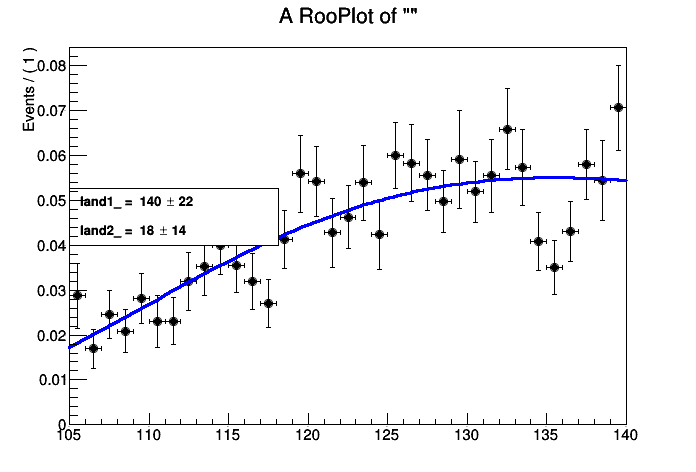
\includegraphics{Figures/RedBkg/fit_zx_ggH_0j_10_200_4e2016.png}}}
    \subfigure [] {\resizebox{5.1cm}{!}{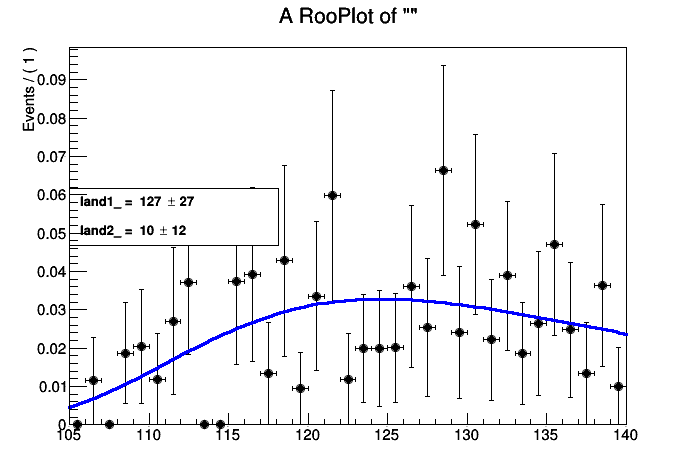
\includegraphics{Figures/RedBkg/fit_zx_ggH_1j_60_120_4mu2016.png}}}
    \subfigure [] {\resizebox{5.1cm}{!}{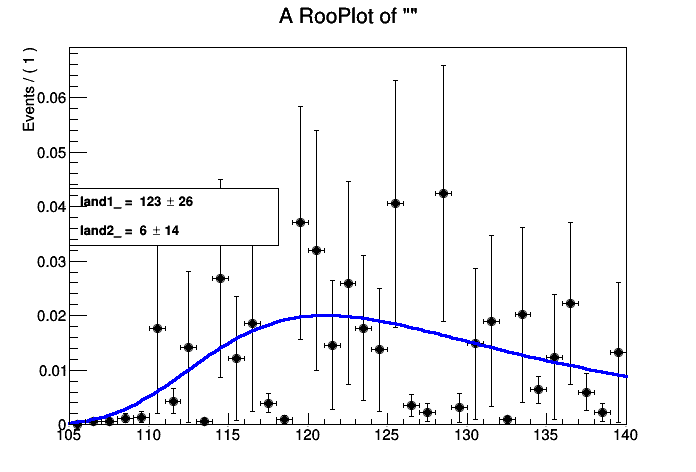
\includegraphics{Figures/RedBkg/fit_zx_VBF_3j_2e2mu2016.png}}}
\caption{Shape of the Z+X background events in the mass range [105, 140] GeV for the ggH$\_$0j$\_10\_200$ category in the $4e$ final state (a), 
for the ggH$\_$1j$\_60\_120$ category in the $4\mu$ final state (b) and for the VBF$\_$2j$\_$mjj$\_$GT350$\_$3j in the $2e2\mu$ final state (c).}
\label{fig:ZXshapesFinal}
\end{center}
\end{figure}

If very low populated categories (less than fifty events selected in the mass window) are considered,
shapes obtained from the inclusive distributions in the given final state are used.
This shape is finally scaled to the yield obtained from the combination of the SS and OS method results. 
The yield uncertainty of ~40$\%$ is able to cover all the discrepancies from the two methods, indeed shape uncertainty is not included. 
%The uncertainty range on the combined estimate is the envelope that covers the uncertainty ranges quoted from the two methods. 
% Figure~\ref{fig:SR_CombinedPrediction}(right) is a visual representation of the predictions of individual methods and the combined results.

\begin{table}[h]
   \centering
   \begin{tabular}{| l | c | c | c |} 
\hline
2016            & 4e                             & $4\mu$                          & $2e2\mu$       \\ 
\hline \hline
Method OS       & 20.2 $\pm$ $6.2_{\rm tot.}$    & 27.0 $\pm$ $8.6_{\rm tot.}$     & 47.7 $\pm$ $10.5_{\rm tot.}$    \\ 
Method SS       & 13.1 $\pm$ $5.5_{\rm tot.}$    & 29.6 $\pm$ $9.0_{\rm tot.}$     & 41.5 $\pm$ $10.3_{\rm tot.}$     \\   
Combined        & 16.1   & 28.2    & 44.4  \\  
\hline
2017            & 4e         & $4\mu$                      & $2e2\mu$       \\ 
\hline \hline
Method OS       & 16.2 $\pm$ $5.0_{\rm tot.}$    & 32.7 $\pm$ $10.3_{\rm tot.}$    & 45.7 $\pm$ $10.2_{\rm tot.}$    \\ 
Method SS       & 10.9 $\pm$ $4.1_{\rm tot.}$    & 33.4 $\pm$ $10.3_{\rm tot.}$    & 40.8 $\pm$ $9.7_{\rm tot.}$    \\   
Combined        & 13.0   & 33.1    & 43.1  \\  
\hline
2018            & 4e         & $4\mu$                      & $2e2\mu$       \\ 
\hline \hline
Method OS       & 25.4 $\pm$ $7.7_{\rm tot.}$    & 50.1 $\pm$ $15.5_{\rm tot.}$    & 67.7 $\pm$ $14.8_{\rm tot.}$    \\ 
Method SS       & 16.1 $\pm$ $5.9_{\rm tot.}$    & 51.9 $\pm$ $15.8_{\rm tot.}$    & 60.7 $\pm$ $14.2_{\rm tot.}$    \\   
Combined        & 19.4   & 50.7    & 63.9  \\  
%Combined Error  &  
%Combined $\kappa_{\rm min}$     & 0.XX  & 0.XX    & 0.XX \\ 
%Combined $\kappa_{\rm max}$     & 0.XX   & 0.XX    & 0.XX \\
\hline
 \end{tabular}
    \caption{
    Summary of the results given by the two methods for the prediction of the contribution of reducible background processes in the signal region for all three years. The weighted mean value of the results of the two methods is taken as the final estimate of this contribution, while the uncertainty of the result covers the uncertainties of both methods. The table shows symmetric individual uncertainties for the two methods, while these are treated as asymmetric in the combination and statistical analysis. Results are given for an integrated luminosity of 35.9, 41.5 and 59.7~fb$^{-1}$ in 2016, 2017 and 2018 data, respectively. 
    }
    \label{tab:reducibleSummary}
\end{table}


% %%%%%%%%%%%%%%%%%%%%%%%
% \begin{figure}[th]
% \begin{center}
% %   \includegraphics{Figures/Shapes_13TeV_zoomed.pdf}
%     \includegraphics[width=0.7\textwidth]{Figures/RedBkg/CombinedPrediction_13TeV.pdf}
% \caption{
% Comparison of the predictions of individual methods and the combined results of two methods (shapes - left,  yields - right). 
% The uncertainty of the result is the one that covers the uncertainties of both methods (asymmetric log-normal distribution). 
% }
% %\label{fig:SR_CombinedShapes}
% \label{fig:SR_CombinedPrediction}
% \end{center}
% \end{figure}
% %%%%%%%%%%%%%%%%%%%%%%%
